%\documentclass[10pt, notes]{beamer}       % print frame + notes
% \documentclass[10pt, notes=only]{beamer}   % only notes
\documentclass[12pt]{beamer}              % only frames

\usetheme[progressbar=frametitle]{metropolis}

\usepackage{booktabs}
\usepackage[scale=2]{ccicons}

\usepackage{pgfplots}
\usepgfplotslibrary{dateplot}

\usepackage{xspace}
\newcommand{\themename}{\textbf{\textsc{metropolis}}\xspace}


% Set up table of contents
\AtBeginSection[]
{
\begin{frame}<beamer>
\frametitle{Outline}
\tableofcontents[
  currentsection,
  sectionstyle=show/shaded,
  subsectionstyle=show/show/hide
]
\end{frame}
}

% Make alert boxes have filled backgrounds
\metroset{block=fill}



\title{Simulation and Theory of Bacterial Transformation}
\date{August 5, 2016}
\author{JD Russo, JJ Dong}
\institute{Department of Physics and Astronomy\\Bucknell University}
%TODO: Add .gif of populations evolving here, or some snazzy graphic

\begin{document}

\maketitle

\section{Introduction}

\subsection{Motivation}
\begin{frame}{Motivation}
  \begin{itemize}
    \item Ubiquitous threat of antibiotic resistance
    \item Main mechanisms of transmission
  \end{itemize}

  \vspace*{\fill}
    \begin{alertblock}{Goal}
      Identify what most significantly affects resistant cell dominance.
    \end{alertblock}
  \vspace*{\fill}

\end{frame}
\note[itemize]{
\item Threat of resistance even in well-controlled diseases (TB)
\item  Main mechanisms of transmission are conjugation and transformation - we focus on transformation
}



\subsection{Biological Background}
%TODO: Label this as Biological Background - Plasmids ?
\begin{frame}[fragile]{Plasmids}
  \begin{itemize}
    \item Small, independently replicating genetic material
    \item Often include DNA segments encoding antibiotic resistance
    \item Imposes a fitness cost on host cell
  \end{itemize}
\end{frame}

\begin{frame}{Transformation and Conjugation}

  \begin{itemize}
    \item \textbf{Transformation:} Cell incorporates plasmid from environment
    \item \textbf{Conjugation:} Plasmid transferred between cells %TODO: Make a similar figure for conjugation
  \end{itemize}

  \vspace*{\fill}
  \centerline{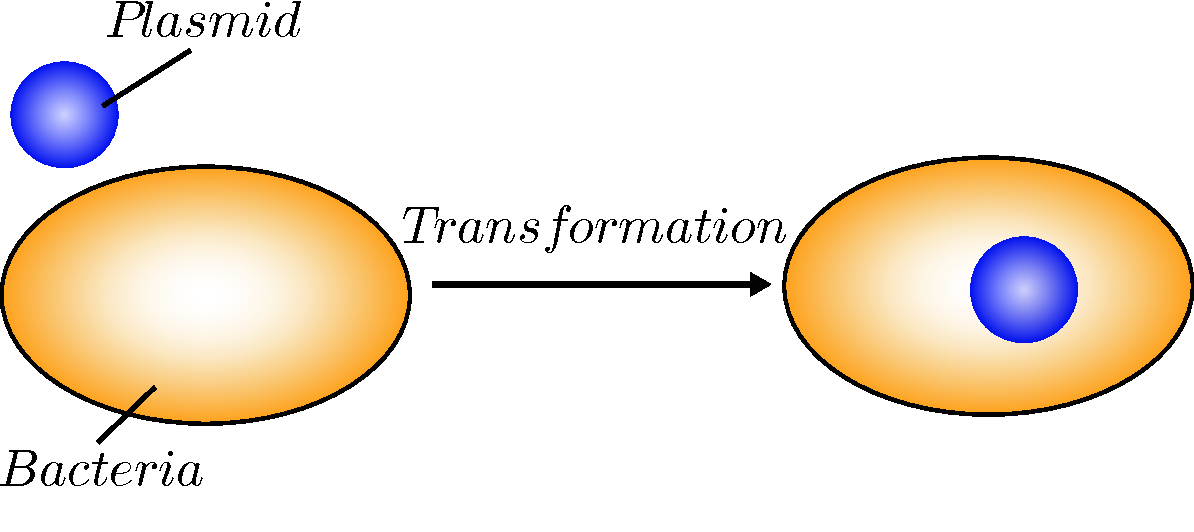
\includegraphics[width=.5\paperwidth]{../../dev/graphics/poster/transformation.pdf}}
  % \vspace*{\fill}
\end{frame}
\note[itemize]{
\item Transformation is the process where a cell incorporates a plasmid from its
environment, translating any encoded genes
\item Conjugation is horizontal transfer of a plasmid between two cells
\item We assume transformation is the primary mechanism of plasmid transfer
%TODO: WHY???
}



\section{Simulation}
%TODO: Should this go here?
\begin{frame}{Simulation vs Modeling}
  \begin{itemize}
  \item Stochastic vs Deterministic
  \item Information about average behavior vs specific system
  \end{itemize}
\end{frame}
\note[itemize]{
\item Mathematical modeling of populations is deterministic - captures info about averages
\item Simulations can incorporate stochastic reactions
\item Individual experiments \"noisily\" follow model
}

% TODO: Add figure of simulated populations over time along with modeled
\begin{frame}{Simulation vs Modeling}

  \begin{align}
    \uncover<1->{&\text{Reaction} & \quad & R \stackrel{\delta}{\longrightarrow} \varnothing \\}
    \uncover<2->{
      &\text{Differential equation}&&\frac{dR}{dt} = - \delta R\\
      &&& R(t) = R_0  e^{- \delta t} \\
    }
    \notag
  \end{align}

  % \vspace*{\fill}
  % \vskip-1.5em %NOTE: This may be necessary if the tags are shown on the hidden equation`
\end{frame}
\note[itemize]{
\item This reaction describes a situation where a resistant cell dies on average every
 $\delta$ time units.
\item When plotted, this describes an exponential function that symptotically
  approaches zero.
\item However, in simulation, this is not a smooth curve. This is a step-like function,
  where at some discrete time the population jumps from one to zero and goes extinct.
}

\subsection{Population Dynamics Model}
\begin{frame}{Population Dynamics Model - %
  \only<1-1>{Constant}%
  \only<2-2>{\color{BurntOrange}Linear}%
  \only<3-3>{\color{Purple}Recycled}}

  \begin{align*}
    \frac{dS}{dt} & = b_S \left(1 - \frac{S + R}{K}\right)S - \alpha
      \only<2->{ \color{BurntOrange}\left( \frac{P}{P_0} \right)}
      \color{black} S \\[0.8ex]
%
    \frac{dR}{dt} & = b_R \left(1 - \frac{S + R}{K}\right)R + \alpha
    \only<2->{\color{BurntOrange}\left( \frac{P}{P_0} \right)}
    \color{black} S - \delta R \\[0.8ex]
%
    \only<2->{
      \color{BurntOrange} \frac{dP}{dt} & \color{BurntOrange} = -\alpha \left( \frac{P}{P_0} \right) S
    }
    \only<3->{\color{Purple} + \delta R}
  \end{align*}

\end{frame}


\subsection{Simulation Methods}


\begin{frame}{Kinetic Monte Carlo Method}
  \begin{itemize}
    \item Initially used to simulation chemical reactions
    \item Captures information about dynamics of a growing system
  \end{itemize}
  \vspace*{\fill}
  % TODO: Make a more detailed flow chart
  \centerline{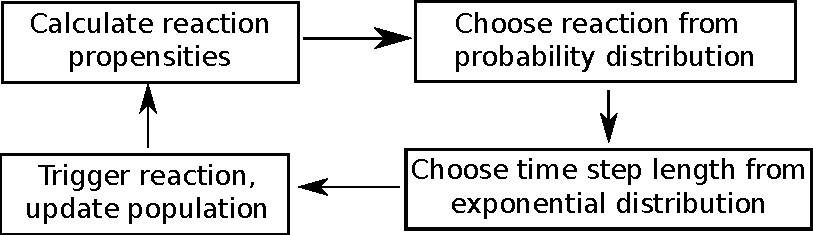
\includegraphics[width=.75\paperwidth]{../../dev/graphics/poster/gillespie.pdf}}
\end{frame}

\note[itemize]{
\item Do I even want to say the part about capturing the dynamics?
}

\begin{frame}[fragile]{Optimizations}
  \begin{itemize}
    \item Sets vs. lists
    \item Occupancy lists
    \item \verb|imshow| vs. \verb|plcolor| %TODO: Does anyone care about this?
  \end{itemize}
\end{frame}




\section{Results}
\subsection{Well-Mixed}
\begin{frame}{Parameter Space}
\end{frame}

\subsection{Lattice}


\section{Conclusions}



\appendix

\begin{frame}[fragile]{Backup slides}
\end{frame}

\begin{frame}[allowframebreaks]{References}
  \bibliography{demo}
  \bibliographystyle{abbrv}
\end{frame}

\end{document}
